\documentclass[a4paper,12pt,rmp,superscriptaddress]{revtex4}
\usepackage{latexsym} 
%\usepackage{helvet}
%\usepackage{times}
%\usepackage[applemac]{inputenc}
\usepackage{setspace}
\usepackage{color}
\usepackage{hyperref}
\usepackage{fancyhdr}
\usepackage{graphicx}
\usepackage{wrapfig}
%%%\usepackage{ulem} % to get the \sout command for editing
\usepackage{amsmath}
\usepackage{amssymb}

% %%% for documents in Italian
% \usepackage[italian]{babel}
% %% accented characters
% \usepackage[T1]{fontenc}
% \usepackage[utf8x]{inputenc}
% %\usepackage[latin1]{inputenc} % -> per windows
% %\usepackage[applemac]{inputenc} % -> per mac


\usepackage[margin=2cm]{geometry}

\bibliographystyle{authordate1}


\begin{document} 

%% a good title is short and defining. 
\title{Piracy in the era of big data: from deep seas to deep web.}

%% author name
\author{Guybrush Threepwood}

%% abstract
% The abstract should be concise and use formal language. A possible
% outline is the following (typically one sentence per bulletpoint).
%
% - Background
%
% - Question / Aims
%
% - Approach
%
% - Results
% - Conclusion
\begin{abstract}
  These notes describe the transformation of illegal acts of sea-borne attack
  and general  drunkenness into illegal acts of commans-line based
  cracking and general nerdiness.  
\end{abstract}

%%% see here for choosing a good title / writing a good abstract
%%% https://www.springer.com/gp/authors-editors/authorandreviewertutorials/writing-a-journal-manuscript/title-abstract-and-keywords/10285522

\maketitle

\setstretch{1}

%%% use \section* and \subsection* for headings wothout numbering
\subsection*{Introduction} 

%% The text is divided into paragraphs 
% Typically a paragraph contains (starts with) a topic sentence. The
% topic sentence should identify the main point of your
% paragraph. Topic sentences should be clear enough that a reader can
% get the gist of your text just by reading the topic sentences of
% each paragraph.
%% 
% Each paragraph should only make one main point. For readability, try
% to keep paragraphs withinx 3-5 sentences. If your paragraph is
% getting too long, it is probably making more than one main point,
% and it may be time to break it into two (and make a new topic
% sentence).
%%


Pirates are criminals who partake in activities such as swordfighting,
treasure hunting and stealing. In order to prove their worth as a
pirate they must pass Three Trials testing their skills in each of the
mentioned skills.  They may also be referred to as buccaneers,
swashbucklers, privateers or corsairs, though in reality these terms
are specific to certain types of pirate.  They are often found on
Caribbean islands and ships.  Scabb Island is the only island where
pirates are free to be pirates.

%%% more than one newline defines a paragraph
%% do not use \\ for line breaks, this will define different types of
%% paragraphs nut there is only one type of paragraph


Rum is an alcoholic beverage made from a sugar plant.  It is a popular
drink among pirates, suitable for being kept on long sea journeys. A
number of kegs could be found on the grassy knoll of the Field of
Honor on Plunder Island.

%%% more than one newline defines a paragraph


We assume that the final volume (in a cycle or subperiod) is a
result of a size-dependent growth and timing
%%% MATH
%%% always use displaymmath or equation for displayed formulas
\begin{displaymath}
  V_f = V_0 \exp \left[ \alpha(V_0)  \tau(V_0)  + \nu \right] \  ,
\end{displaymath}
%%% use $$ for in line formulas
where $V_x$ is volume and $\alpha$ and $\tau $ quantify the duration
and growth in the period (or cell cycle). $\nu$ is noise.  Note that
there is no hypothesis of exponential growth rate, just that growth
during a period is represented as en effective exponential growth
(this is formally always possible, and physically it is justified by
the mean time traces).


%%% Figure
\begin{figure}[htbp]
  \centering
  %%% using pdflatex you can include pdf jpg and png files
   \includegraphics[width=0.5\textwidth]{plot1}
   %%% see here for how to write a figure caption
   %% https://blog.bioturing.com/2018/05/10/how-to-craft-a-figure-legend-for-scientific-papers/
   % Figure captions should be standalone, i.e., descriptive enough to
   % be understood without having to refer to the main text. Effective
   % captions typically include the following elements:
%
   % (1) a declarative title that summarises the result or major
   % finding of the data you are presenting in the figure;
%
   % (2) a brief description of the methods necessary to understand
   % the figure without having to refer to the main text;
%
   % (3) technical information, for example, number of simulations,
   % asterisks denoting P-values etc.
   \caption{There is an interplay between growth and timing
     control. Assuming the linear response framework, we measured
     $\lambda$ and $\gamma$ inferring
     $\eta$ indirectly. For bacteria, all three parameters are
     measurable.  Eukaryotes are adder-like and generally control
     division through a vatiable mix of growth and timing. Some
     bacteria show the expected behavior $eta \simeq 0$ $\lambda
     \simeq 1/2$. Some other points are scattered, especially for
     bacteria.  }
%%% always refer to figures from the text using \label and  \ref
   \label{fig:1}
\end{figure}

This relation shows that noise in growth rate leads to an overestimate
of the control due to timing, and hence to an overestimate of the
slope subracted to $\lambda$ in order to measure $\eta$ in
%%% always refer to figures from the text using \label and  \ref
Figure~\ref{fig:1}. We can try to evaluate more carefully this
contribution. Note that $\eta$ (slope of growth rate vs size
fluctuation conditional average) can be measured directly in the data.


%%% always use displaymath or equation for displayed formulas
\begin{displaymath}
  q_f - q_0 = G(V_0) + \nu
\end{displaymath}
where $q_x = \log(V_x)$ and $G(V_0) \alpha(V_0) \tau(V_0)$ and 
%
$q_f - q_0 = \log\frac{V_f}{V_0}$ so the previous equation is just the
size-growth plot.  We now can measure two things. First, the
conditional average of the net growth given the log initial volume,
i.e., the size-growth plot
%
\begin{displaymath}
  G(V_0) = \langle G \rangle - \lambda (q_0 - \langle q_0 \rangle) 
\end{displaymath}
%
$\lambda$, the slope of the size-growth plot measures the strength of
the control. For the full cell cycle, $\lambda = 1/2$ is an adder.

%%% more than one newline defines a paragraph


Second, the correction due to timing, i.e., the conditional average of
timing vs log size
\begin{displaymath}
  \tau(V_0) = \langle \tau \rangle - \gamma (q_0 - \langle q_0
  \rangle) \ .
\end{displaymath}




\subsection*{Control on $\alpha$ in bacteria}

To proceed in this direction,  we can write, in general, that 
\begin{displaymath}
  \alpha(V_0) = 
   \langle \alpha \rangle - (\xi + \eta) \delta_q \ ,
\end{displaymath}
and, in data (for bacteria, where this is available) evaluate $\xi +
\eta$ from the plot of $\alpha$ vs $\delta_q$, then evaluate $\eta$
from the plot of $ \frac{\langle G \rangle}{\langle \tau \rangle}$ vs
$\delta_q$ and test whether there is a difference. The paragraphs
below discuss in more detail the relation between these variables,
accounting for noise in growth rate $\alpha$.

%%% more than one newline defines a paragraph



Elaine Marley–Threepwood was the Governor of the Tri-Island Area. Her
gubernatorial powers covered Mêlée Island, Booty Island and Plunder
Island though she had some influence in a number of other locations
too.

She was an able sailor and a captain of her own ship and crew. She was
a resourceful and intelligent woman. She became the object of
obsession by the zombie pirate LeChuck, which led her into situations
where she fell into becoming the damsel in distress. More often than
not however, she was perfectly capable of escaping and handling
herself. In combat, she was an accomplished swordswoman and could
throw a rather dangerous punch.


\end{document}


%%% Local Variables: 
%%% mode: latex
%%% TeX-master: t
%%% End:
